\documentclass{standalone}

\usepackage{tikz}
\usetikzlibrary{decorations.markings}
\usetikzlibrary{arrows.meta}
\usetikzlibrary{calc}

\usepackage{amsmath}

\begin{document}


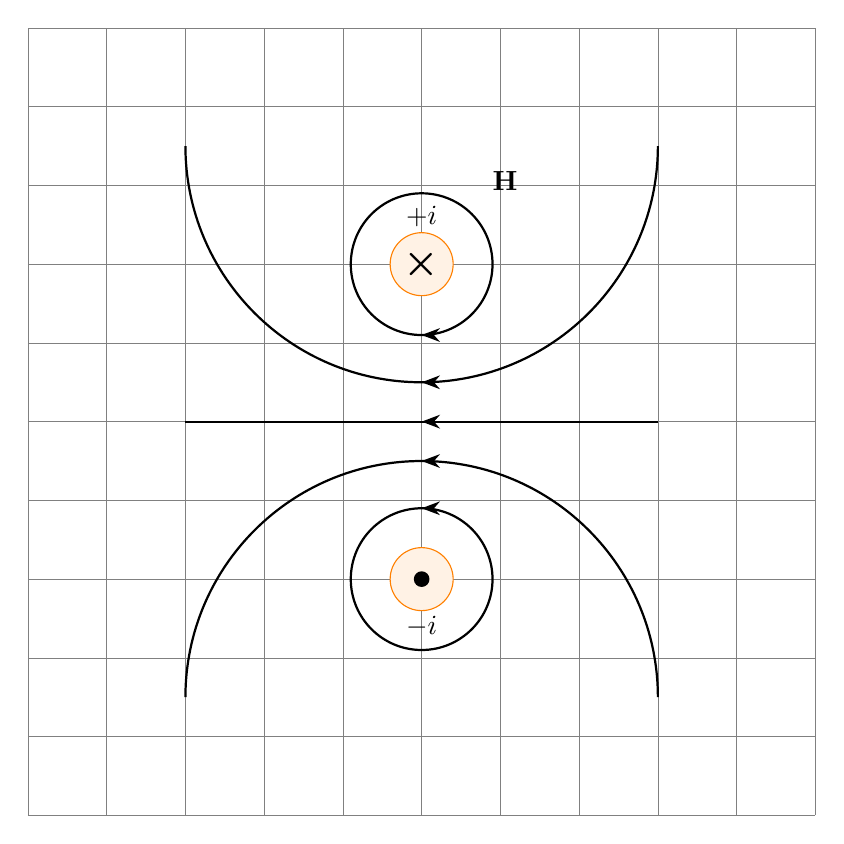
\begin{tikzpicture}

\draw[help lines] grid (10,10);

%position of bottom wire
\coordinate (A1) at (5,3);

%position of top wire
\coordinate (A2) at (5,7);


% node with negative charge
\draw[fill=orange!10, draw=orange] (A1) circle[radius=0.4] node[below of=A1, yshift=0.4cm] {$-i$};
\node[circle, fill=black, inner sep=2pt]  at (A1) {};

% node with positive charge
\draw[fill=orange!10, draw=orange] (A2) circle[radius=0.4] node[above of=A2, yshift=-0.4cm] {$+i$};
\node at (A2) {\Large$\boldsymbol{\times}$};

% magnetic field lines
\draw[thick, postaction={decorate}, decoration={markings, mark=at position 0.5 with {\arrowreversed{Stealth}}}] (2,8.5) arc
(-180:0:3cm and 3cm);
\draw[thick, postaction={decorate}, decoration={markings, mark=at position 0.75 with {\arrowreversed{Stealth}}}] (5,7)
circle[radius=0.9];
\draw[thick, postaction={decorate}, decoration={markings, mark=at position 0.5 with {\arrow{Stealth}}}] (8,5) -- (2,5);
\draw[thick, postaction={decorate}, decoration={markings, mark=at position 0.5 with {\arrowreversed{Stealth}}}] (2,1.5) arc
(180:0:3cm and 3cm);
\draw[thick, postaction={decorate}, decoration={markings, mark=at position 0.25 with {\arrow{Stealth}}}] (5,3)
circle[radius=0.9];

\node at ($(A2)+(45:1.5)$) {$\textbf{H}$};

\end{tikzpicture}


\end{document}